\documentclass[border=2pt,tikz]{standalone}
\usepackage{xcolor}
\definecolor{databoxfill}{rgb}{0.90,0.90,0.90}
\definecolor{databoxdraw}{rgb}{0.45,0.45,0.45}
\definecolor{attackboxfill}{rgb}{0.99,0.93,0.93}
\definecolor{attackboxdraw}{rgb}{0.60,0.00,0.00}
\definecolor{defenseboxfill}{rgb}{0.93,0.93,0.99}
\definecolor{defenseboxdraw}{rgb}{0.00,0.00,0.60}
\definecolor{metricboxfill}{rgb}{0.92,0.97,0.92}
\definecolor{metricboxdraw}{rgb}{0.00,0.45,0.00}
\definecolor{flowdraw}{rgb}{0.25,0.25,0.25}
\definecolor{flowdashdraw}{rgb}{0.45,0.45,0.45}
\usepackage{tikz}
\usetikzlibrary{positioning,arrows.meta,shapes.geometric,fit,backgrounds}
\begin{document}
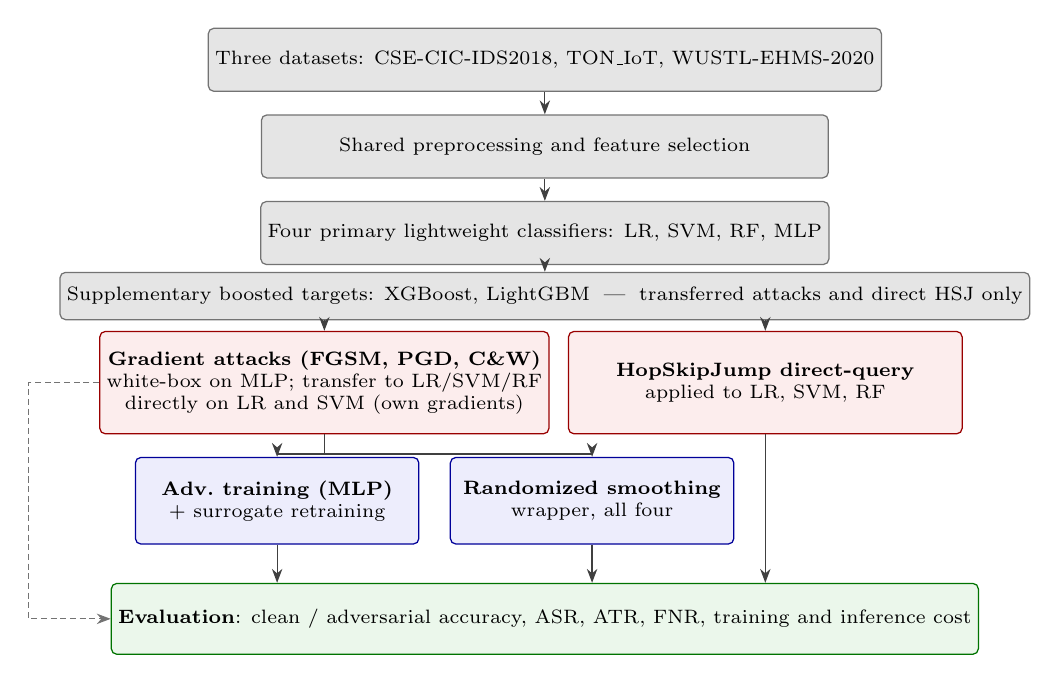
\begin{tikzpicture}[
  >=Stealth,
  font=\scriptsize,
  every node/.style={align=center, inner sep=2.5pt, font=\scriptsize},
  databox/.style    ={rectangle, rounded corners=2pt, draw=databoxdraw,   line width=0.45pt, fill=databoxfill,   minimum height=8mm,  minimum width=72mm},
  attackbox/.style  ={rectangle, rounded corners=2pt, draw=attackboxdraw, line width=0.45pt, fill=attackboxfill, minimum height=13mm, minimum width=50mm},
  defensebox/.style ={rectangle, rounded corners=2pt, draw=defenseboxdraw,line width=0.45pt, fill=defenseboxfill,minimum height=11mm, minimum width=36mm},
  metricbox/.style  ={rectangle, rounded corners=2pt, draw=metricboxdraw, line width=0.45pt, fill=metricboxfill, minimum height=9mm,  minimum width=108mm},
  flow/.style       ={->, line width=0.45pt, draw=flowdraw},
  flowdash/.style   ={->, line width=0.45pt, draw=flowdashdraw, dash pattern=on 2.2pt off 1.3pt}
]

\node[databox] (data) at (0,  5.4) {Three datasets: CSE-CIC-IDS2018, TON\_IoT, WUSTL-EHMS-2020};
\node[databox] (prep) at (0,  4.3) {Shared preprocessing and feature selection};
\node[databox] (mods) at (0,  3.2) {Four primary lightweight classifiers: LR, SVM, RF, MLP};

\node[attackbox] (grad) at (-2.8, 1.3)
   {\textbf{Gradient attacks (FGSM, PGD, C\&W)}\\white-box on MLP; transfer to LR/SVM/RF\\directly on LR and SVM (own gradients)};
\node[attackbox] (hsj)  at ( 2.8, 1.3)
   {\textbf{HopSkipJump direct-query}\\applied to LR, SVM, RF};

\node[databox, minimum width=108mm, minimum height=6mm] (supp) at (0, 2.40)
   {Supplementary boosted targets: XGBoost, LightGBM \;---\; transferred attacks and direct HSJ only};

\node[defensebox] (atrain) at (-3.4, -0.2)
   {\textbf{Adv.\ training (MLP)}\\+ surrogate retraining};
\node[defensebox] (rs)     at ( 0.6, -0.2)
   {\textbf{Randomized smoothing}\\wrapper, all four};

\node[metricbox] (eval) at (0, -1.7)
   {\textbf{Evaluation}: clean / adversarial accuracy, ASR, ATR, FNR, training and inference cost};

\draw[flow] (data) -- (prep);
\draw[flow] (prep) -- (mods);

\draw[flow] (mods.south) -- (supp.north);
% drop straight into each attack box from the point directly above it,
% rather than fanning out from a single point on the band
\draw[flow] (supp.south -| grad.north) -- (grad.north);
\draw[flow] (supp.south -| hsj.north) -- (hsj.north);

\draw[flow] (grad.south) -- ++(0,-2.5mm) -| (atrain.north);
\draw[flow] (grad.south) -- ++(0,-2.5mm) -| (rs.north);

\draw[flow] (atrain.south) -- (atrain.south |- eval.north);
\draw[flow] (rs.south)     -- (rs.south     |- eval.north);

\draw[flow] (hsj.south) -- (hsj.south |- eval.north);

\draw[flowdash] (grad.west) -- ++(-9mm,0) |- (eval.west);

\end{tikzpicture}
\end{document}
